\documentclass{ximera}

\addPrintStyle{..}

\begin{document}
	\author{Bart Lambregs}
	\xmtitle{Gravitationele potentiële energie, algemeen}{}
    \xmsource\xmuitleg


	\subsection{Gravitationele potentiële energie, algemeen}

	Beschouw een massa onderhevig aan de universele gravitatiekracht. We gaan opnieuw opzoek naar een potentiële energiefunctie geassocieerd aan deze kracht.
	\begin{image}
	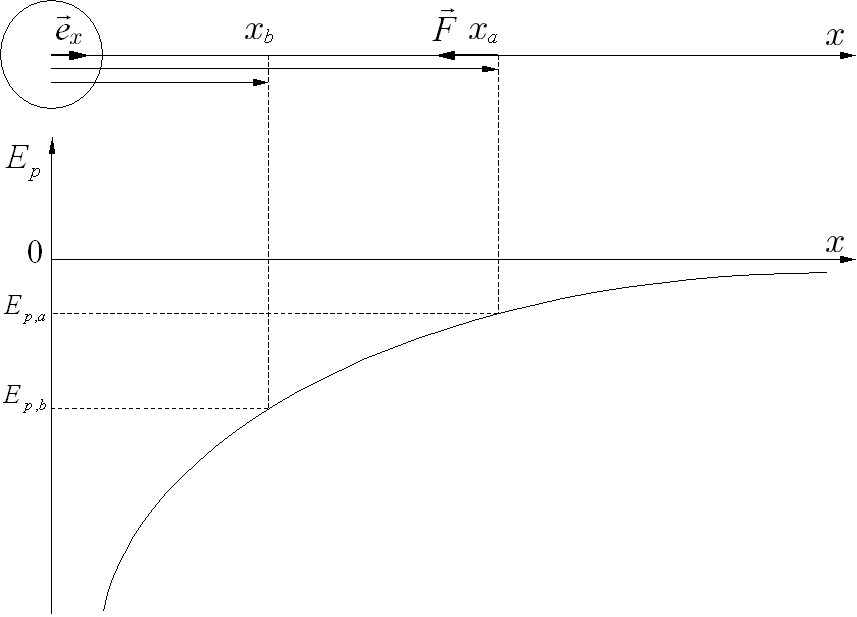
\includegraphics[width=0.9\textwidth ,angle=0]{gravitationele_energie_algemeen}
	\end{image}
	
	Kiezen we een $x$-as met de oorsprong op de massa $m$ dan wordt, omdat de kracht steeds naar de oorsprong is gericht, de component van de universele gravitatiekracht op de massa $m'$ gegeven door
	\begin{eqnarray*}
	F(x)&=&-G\frac{mm'}{x^2}
	\end{eqnarray*}
	De arbeid die door de gravitatiekracht wordt geleverd bij de verplaatsing van de massa $m'$ van $x_a$ naar $x_b$ wordt dan:
	\begin{eqnarray*}
	W&=&\int_{x_a}^{x_b}-G\frac{mm'}{x^2}~{\rm d}x\\
	&=&-Gmm'\int_{x_a}^{x_b}\frac{1}{x^2}~{\rm d}x\\
	&=&-Gmm'\left[-\frac{1}{x}\right]_{x_a}^{x_b}\\
	&\Updownarrow&\\
	W&=&\left(-G\frac{mm'}{x_a}\right)-\left(-G\frac{mm'}{x_b}\right)
	\end{eqnarray*}
	De potentiële energie voor een massa $m'$ wordt bijgevolg geven
	door
	\begin{eqnarray}
	E_p&=&-G\frac{mm'}{x}
	\end{eqnarray}
	
\end{document}
